\section{A Methodology for Using Energyplus}\label{a-methodology-for-using-energyplus}

This section provides a step by step outline that will help you streamline creating your building models for using EnergyPlus.

\subsection{\emph{Step 1}: Plan Ahead}\label{step-1-plan-ahead}

Some preliminary steps will facilitate the construction of your input file. EnergyPlus requires some information in specified, externally available formats; other information may require some lead time to obtain. The following checklist should be completed before you start to construct your input file.

\begin{itemize}
\item
  Obtain location and design climate information for the city in which your building is located. If possible, use one of the weather files available for your weather period run.
\item
  Obtain sufficient \emph{building} \emph{construction} information to allow specification of overall building geometry and surface constructions (including exterior walls, interior walls, partitions, floors, ceilings, roofs, windows and doors).
\item
  Obtain sufficient \emph{building} \emph{use} information to allow specification of the lighting and other equipment (e.g.~electric, gas, etc.) and the number of people in each area of the building.
\item
  Obtain sufficient \emph{building} \emph{thermostatic} \emph{control} information to allow specification of the temperature control strategy for each area of the building.
\item
  Obtain sufficient \emph{HVAC} \emph{operation} information to allow specification and scheduling of the fan systems.
\item
  Obtain sufficient \emph{central plant} information to allow specification and scheduling of the boilers, chillers and other plant equipment.
\end{itemize}

\subsection{\emph{Step 2}: ``Zone" the Building}\label{step-2-zone-the-building}

A building ``surface'' is the fundamental element in the building model. In the general sense, there are two types of ``surfaces'' in EnergyPlus. These are:

1.~~ heat transfer surfaces~ and

2.~~ heat storage surfaces

The first rule of building modeling is, ``\emph{Always define a surface as a heat storage surface unless it must be defined as a heat transfer surface}''. Any surface, which is expected to separate spaces of significantly different temperatures, must be defined as a \emph{heat transfer surface.} Thus, exterior surfaces, such as outside walls, roofs and floors, are \emph{heat transfer surfaces}. Interior surfaces (partitions) are \emph{heat storage surfaces} if they separate spaces maintained at the same temperature and \emph{heat transfer surfaces} if they separate spaces maintained at different temperatures. A discussion of how to define heat transfer and heat storage surfaces will occur in later steps. In order to correctly ``zone'' the building it is necessary only to distinguish between the two.

\begin{figure}[hbtp] % fig 12
\centering
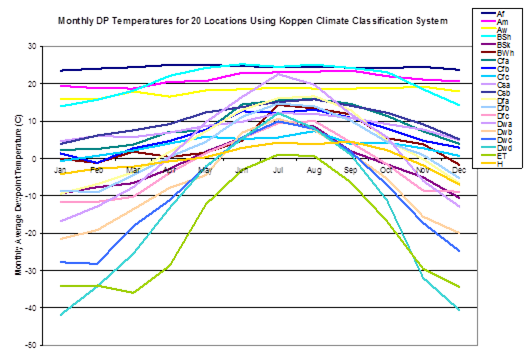
\includegraphics[width=0.9\textwidth, height=0.9\textheight, keepaspectratio=true]{media/image012.png}
\caption{Adult Education Center \protect \label{fig:adult-education-center}}
\end{figure}

A ``zone'' is a \emph{thermal}, not a \emph{geometric}, concept. A ``zone'' is an air volume at a uniform temperature plus all the heat transfer and heat storage surfaces bounding or inside of that air volume. EnergyPlus calculates the energy required to maintain each zone at a specified temperature for each hour of the day. Since EnergyPlus performs a zone heat balance, the first step in preparing a building description is to break the building into zones. The objective of this exercise is to define as \emph{few} zones as possible without significantly compromising the integrity of the simulation.

Although defining building zones is somewhat of an art, a few general rules will keep the new simulation user out of trouble. Consider Figure~\ref{fig:adult-education-center} which shows the floor plan of an Adult Education Center.

The question is, ``How many \emph{thermal} zones should be used to model this building?''~ The inexperienced building modeler may be tempted to define each room in the building as a zone, but the thermal zone is defined as a volume of air at a uniform temperature. The general rule then is to \emph{use the number of fan systems (and radiant systems) not the number of rooms to determine the number of zones in the building.} The minimum number of zones in a general simulation model will usually be equal to the number of systems serving the building. The collection of heat transfer and heat storage surfaces defined within each zone will include all surfaces bounding or inside of the space conditioned by the system.

\subsection{Zoning -- Concept 1 - Simple}\label{zoning-concept-1---simple}

Complete estimates of the total building load (magnitude only) may be obtained with very simple models. For example the total building load calculated using a one-zone model of the Education Center (Figure~\ref{fig:single-zone-model-of-the-adult-education}) will \textbf{NOT} be significantly different from the total building load calculated using a more detailed model. The \emph{distribution} of the load within the building cannot be estimated with the simplified building model, but its \emph{magnitude} (such as would be used in sizing the central plant equipment) can be quickly estimated using a very simple model. For simplicity, assume there is no ground heat transfer; if you want to simulate ground heat transfer, you should use the slab and/or basement programs as described in the Auxiliary Programs document.

\begin{figure}[hbtp] % fig 13
\centering
\includegraphics[width=0.9\textwidth, height=0.9\textheight, keepaspectratio=true]{media/image013.png}
\caption{Single Zone Model of the Adult Education Center. \protect \label{fig:single-zone-model-of-the-adult-education}}
\end{figure}

\subsection{Zoning -- Concept 2 - Detailed}\label{zoning-concept-2---detailed}

A more detailed model will allow you to determine more accurately the actual distribution of loads/energy within the building. In a more detailed model of the education center, five systems were designed to serve the Adult Education Center. These systems with the thermal zones they serve are shown in the table below. The location of each zone is shown in accompanying figure.

% table 2
\begin{longtable}[c]{@{}lllll@{}}
\caption{Zoning the Building by System Type. \label{table:zoning-the-building-by-system-type.}} \tabularnewline
\toprule 
System Number & System Name & CFM & m/s & Zone Served \tabularnewline
\midrule
\endfirsthead

\caption[]{Zoning the Building by System Type.} \tabularnewline
\toprule 
System Number & System Name & CFM & m/s & Zone Served \tabularnewline
\midrule
\endhead

1 & Four Pipe Fan Coil & 3900 & 19.812 & Zone 1 \tabularnewline
1 & Four Pipe Fan Coil & 2500 & 12.7 & Zone 2 \tabularnewline
2 & Single Zone Draw Through & 1400 & 7.112 & Zone 3 \tabularnewline
3 & Single Zone Draw Through & 2250 & 11.43 & Zone 5 \tabularnewline
4 & Single Zone Draw Through & 2450 & 12.446 & Zone 6 \tabularnewline
5 & Unit Heater & 185 & .9398 & Zone 4 \tabularnewline
5 & Unit Heater & 41 & .20828 & Zone 7 \tabularnewline
\bottomrule
\end{longtable}

Take note of Zone 1, Zone 2, Zone 4, and Zone 7 in Figure~\ref{fig:thermal-zones-in-the-education-center}. The two important zoning concepts can be demonstrated with the zoning to reinforce the idea of a thermal zone and encourage the use of simplified models.

\begin{figure}[hbtp] % fig 14
\centering
\includegraphics[width=0.9\textwidth, height=0.9\textheight, keepaspectratio=true]{media/image014.png}
\caption{Thermal Zones in the Education Center \protect \label{fig:thermal-zones-in-the-education-center}}
\end{figure}

1.~~ Notice that Zones 4 and 7 include two rooms that are not adjacent to one another but are served by the same system. Because the air temperature in the two spaces is maintained at the same uniform temperature, the two spaces, though separated spatially, may be defined as a single zone. For our purposes, we will define them as separate zones.

2.~~ Notice that Zone 1 and Zone 2 are served by the same fan system and could be defined as a single zone with 7650 cfm of conditioned air supplied to the space. The space was split into two zones because the designer expected higher solar loads on the South and West sides of the wing and wanted to examine the \emph{distribution} as well as the \emph{magnitude} of the load in the space.

\subsection{\emph{Step 3}: Prepare to Construct the Building Model}\label{step-3-prepare-to-construct-the-building-model}

Working from blueprints or sketches and following the guidelines in Step 2, the building zones were determined. It is recommended that the engineer sketch the building with its zones. Surface dimensions should be included in the sketch. Additional geometric and surface information is required before an input file describing the building can be constructed. Specifically the building model must:

1.~~ Determine \emph{heat transfer} and \emph{heat storage} surfaces.

2.~~ Define equivalent surfaces.

3.~~ Specify surfaces and subsurfaces (windows, doors, etc.) construction and materials.

4.~~ Compile surface and subsurface information.

By the way, the file for this example, the 1 zone model are contained in your EnergyPlus installation ExampleFiles\textbackslash{}BasicFiles folder.

\subsubsection{Step 3.1.~~~~~ Determine heat transfer and heat storage surfaces.}\label{step-3.1.-determine-heat-transfer-and-heat-storage-surfaces.}

The surfaces of the building can be described in any order; grouping surfaces by zone may help you read the input file. Specifics of the describing surfaces help categorize the surface's heat transfer/storage as well as identify the surface construction information.

The details of inputting surfaces are described in the Input/Output Reference document. The allowable surface types are shown in the following table:

% table 3
\begin{longtable}[c]{p{1.91in}p{4.08in}}
\caption{Surface types and categorization \label{table:surface-types-and-categorization}} \tabularnewline
\toprule 
Surface Type & Applicability \tabularnewline
\midrule
\endfirsthead

\caption[]{Surface types and categorization} \tabularnewline
\toprule 
Surface Type & Applicability \tabularnewline
\midrule
\endhead

BuildingSurface:Detailed & Wall, Roof, Ceiling, Floor \tabularnewline
FenestrationSurface:Detailed & Window, Door, Glassdoor \tabularnewline
InternalMass & Areas internal to a zone \tabularnewline
Shading:Site:Detailed & Shading devices external to the building face (other buildings, trees, etc.) \tabularnewline
Shading:Zone:Detailed & Shading devices attached to the building (overhang, fin) \tabularnewline
\bottomrule
\end{longtable}

The pieces of the definition that designate BuildingSurface:Detailed surfaces as either \emph{heat transfer} or \emph{heat storage} surfaces are:

\begin{lstlisting}

  A5 , \field Outside Boundary Condition
         \required-field
         \type choice
         \key Surface
         \key Zone
         \key Space
         \key Outdoors
         \key Ground
         \key OtherSideCoefficients
         \key OtherSideConditionsModel
    A6,  \field Outside Boundary Condition Object
         \type object-list
         \object-list OutFaceEnvNames
         \note Non-blank only if the field Outside Boundary Condition is Surface, Zone, Space, OtherSideCoefficients,
         \note or OtherSideConditionsModel
         \note If Surface, specify name of corresponding surface in adjacent zone or
         \note specify current surface name for internal partition separating like zones
         \note If Zone, specify the name of the corresponding zone and
         \note the program will generate the corresponding interzone surface
         \note If OtherSideCoefficients, specify name of SurfaceProperty:OtherSideCoefficients
         \note If OtherSideConditionsModel, specify name of SurfaceProperty:OtherSideConditionsModel
    A7 , \field Sun Exposure
         \required-field
         \type choice
         \key SunExposed
         \key NoSun
         \default SunExposed
    A8,  \field Wind Exposure
         \required-field
         \type choice
         \key WindExposed
         \key NoWind
         \default WindExposed
\end{lstlisting}

Note that subsurfaces (windows, doors) on these base surfaces will inherit the base surface properties listed above. The following examples will use a bit more of the Surface definition to give context.

Surfaces that specify ``themselves'' as the outside boundary condition are ceilings, floors and partitions that divide temperature-controlled spaces. The program assumes that the surface temperatures on both sides of the surface are the same. This means that even though heat may be stored in a partition, ceiling, or floor, no heat flows \emph{through} it.

Heat Storage Surfaces (Use current Surface name for ExteriorEnvironment), e.g.:

\begin{lstlisting}

BuildingSurface:Detailed,Zn005:Wall006,  !- Base Surface Name
    Wall,INTERIOR,  !- Class and Construction Name
    MAINE WING,  !- Zone
    Surface, Zn005:Wall006,  !- Exterior Conditions and Target
     NoSun,  !- Solar Exposure
     NoWind,  !- Wind Exposure
    0.5000000    ,  !- VF to Ground
             4, !-Rectangle
     57.90000    ,   57.79000    ,   10.00000    ,
     57.90000    ,   57.79000    ,  0.0000000E+00,
     57.90000    ,   47.79000    ,  0.0000000E+00,
     57.90000    ,   47.79000    ,   10.00000    ;
\end{lstlisting}

Some surfaces divide the temperature controlled space from the outside environment. Surfaces that are both sun and wind exposed (e.g.~exterior walls, exposed floors, roofs) feel the full effect of both solar radiation and outside temperature, and the outside air film resistance for these surfaces changes with wind speed and wind direction. Surfaces that are not sun or wind exposed (a wall to an ``uncontrolled'' space) are not affected by solar radiation, wind speed or direction and have a constant outside convective air film resistance.

Heat Transfer Surfaces Exposed to the Outside Environment, such as Exterior Walls, Roofs, Exposed Floors:

\begin{lstlisting}

BuildingSurface:Detailed,Zn005:Wall002,  !- Base Surface Name
    Wall,EXTERIOR,  !- Class and Construction Name
    MAINE WING,  !- Zone
    Outdoors,,  !- Exterior Conditions and Target (if applicable)
     SunExposed,  !- Solar Exposure
     WindExposed,  !- Wind Exposure
    0.5000000    ,  !- VF to Ground
             4, !-Rectangle
     77.90000    ,   47.79000    ,   10.00000    ,
     77.90000    ,   47.79000    ,  0.0000000E+00,
     77.90000    ,   67.79000    ,  0.0000000E+00,
     77.90000    ,   67.79000    ,   10.00000    ;
\end{lstlisting}

Surfaces such as basement walls and slab floors separate the space from the earth surrounding the surfaces. Therefore, the outside surface temperatures become the ground temperatures.

Heat Transfer Surfaces in Contact with the Ground, such as Basement Walls or Slab Floors:

\begin{lstlisting}

BuildingSurface:Detailed,Zn004:Flr001,  !- Base Surface Name
    Floor,SLAB FLOOR,  !- Class and Construction Name
    ARIZONA WING,  !- Zone
    Ground,,  !- Exterior Conditions and Target (if applicable)
     NoSun,  !- Solar Exposure
     NoWind,  !- Wind Exposure
     1.000000    ,  !- VF to Ground
             4, !-Rectangle
     38.01000    ,   8.510000    ,  0.0000000E+00,
     18.01000    ,   8.510000    ,  0.0000000E+00,
     18.01000    ,   28.51000    ,  0.0000000E+00,
     38.01000    ,   28.51000    ,  0.0000000E+00;
\end{lstlisting}

Other surfaces separate zones that may be at different temperatures. These surface types allow heat transfer (by conduction through the walls) from a zone at a higher temperature to a zone at a lower temperature. The location of the heat storage surface in the zone is not important except in specialized solar studies. The surface above (wall to uncontrolled space) would be more correctly modeled as an interzone surface.

Heat Transfer Surfaces Exposed to Another Zone, such as Interzone walls, ceilings or floors:

\begin{lstlisting}

BuildingSurface:Detailed,Zn005:Wall005,  !- Base Surface Name
    Wall,INTERIOR,  !- Class and Construction Name
    MAINE WING,  !- Zone
    Surface,Zn001:Wall009,  !- Exterior Conditions and Target
     NoSun,  !- Solar Exposure
     NoWind,  !- Wind Exposure
    0.5000000    ,  !- VF to Ground
             4, !-Rectangle
     57.90000    ,   47.79000    ,   10.00000    ,
     57.90000    ,   47.79000    ,  0.0000000E+00,
     67.90000    ,   47.79000    ,  0.0000000E+00,
     67.90000    ,   47.79000    ,   10.00000    ;
   
\end{lstlisting}

\subsubsection{Step 3.2.~~~~ Define equivalent surfaces as desired.}\label{step-3.2.-define-equivalent-surfaces-as-desired.}

When the building was zoned, our objective was to define as \emph{few} zones as possible. Now we would like to extend this objective to include defining as \emph{few} surfaces as possible without significantly compromising the integrity of the simulation. We reduce the number and complexity of surfaces in our input file by defining \emph{equivalent} surfaces.

Before dealing with equivalent surfaces, it is appropriate to take the concept of a thermal zone one step further. EnergyPlus performs heat balances on individual zone surfaces and on the zone air. For purposes of the heat transfer calculations, a \emph{geometrically} correct rendering of the zone surfaces is not required. The surfaces do not even have to be connected. As long as the program knows to which thermal zone (mass of air) each surface transfers heat, it will calculate all heat balances correctly. For example, all heat storage surfaces of the same construction within a zone may be defined as a single rectangular surface. The size of this \emph{equivalent} surface will equal the sum of all the areas of all the heat storage surfaces in the zone. A few simple rules will further explain what we mean by \emph{equivalent} surfaces and how these surfaces may be used. Remember that these are guidelines for optional simplification of input. Each simplification must be evaluated to determine if it would significantly impact certain shading, interior solar gains, or daylighting features. The goal is to seek an adequate level of detail to capture the key features of the building envelope without spending excess time describing and computing results for details that are insignificant.

1.~~ \emph{Define all roofs and floors as rectangles regardless of the shape of the zone.} Each zone may have one rectangular roof and one rectangular floor of a given construction.

2.~~ \emph{Define all heat storage surfaces of the same construction within a zone as a single surface}. The size of the single surface is obtained by summing the individual surface areas exposed to the zone. Thus, if a partition is completely within a zone (both sides of the partition are exposed to the zone), the area of each side must be added to the area of the equivalent surface. On the other hand, if the partition separates two zones, the area of only one side should be added to the equivalent surface.

3.~~ \emph{Combine all windows on a given exterior surface into a single window}. Usually each exterior surface should have only one window of each type. Overhangs or other shading devices may require that more windows be specified or combined together. By using the WindowMaterial:Glazing construction for your glass door, they will be correctly modeled in EnergyPlus with sunlight transferring into the zone.

The following figure shows the surfaces and subsurfaces required for a one-zone model, i.e., the education center. Since there were two types of partitions in the building, two heat storage surfaces (``internal mass'') of different constructions were defined.

\begin{figure}[hbtp] % fig 15
\centering
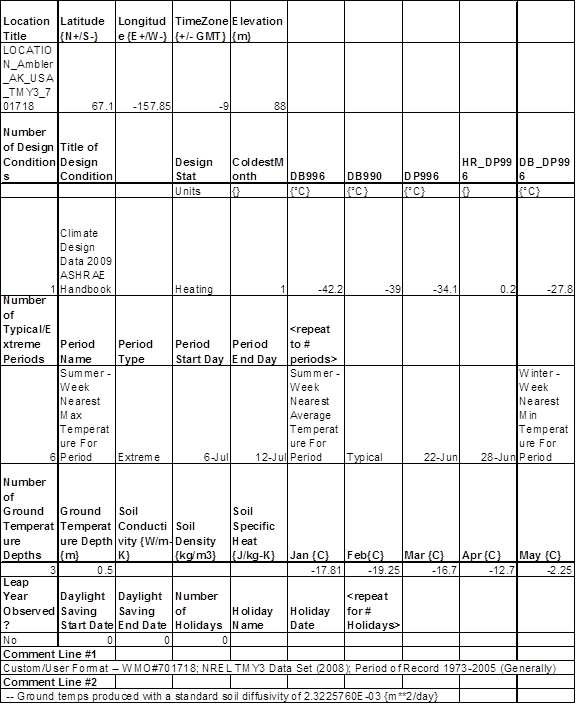
\includegraphics[width=0.9\textwidth, height=0.9\textheight, keepaspectratio=true]{media/image015.png}
\caption{Simplifications Using Equivalent Surfaces \protect \label{fig:simplifications-using-equivalent-surfaces}}
\end{figure}

\subsubsection{Step 3.3. Specify construction elements}\label{step-3.3.-specify-construction-elements}

BLAST, DOE-2 and other programs often have ``libraries'' of constructions, schedules, and other aspects of simulating the building. In EnergyPlus, we have a special set of files in the DataSets folder that represent many facets of building simulation. Data sets are usually IDF snippets or macro files. For constructions, using the guidelines in the ASHRAE Handbook of Fundamentals (2005), the file ASHRAE\_2005\_HOF\_Materials.idf contains materials and constructions from Chapters 30 and 25. Since Chapter 30 discusses heating and cooling loads, it includes constructions for light, medium and heavy weight buildings -- these constructions are represented in the dataset file. For the education center, ``medium'' constructions are used. For the windows, we will use the Double Pane Window from the previous exercise.

% table 4
\begin{longtable}[c]{@{}lll@{}}
\caption{Building Elements \label{table:building-elements}} \tabularnewline
\toprule 
Type (1) & Name (2) & Material (3) \tabularnewline
\midrule
\endfirsthead

\caption[]{Building Elements} \tabularnewline
\toprule 
Type (1) & Name (2) & Material (3) \tabularnewline
\midrule
\endhead

Wall & Medium Exterior Wall & M01 100mm brick \tabularnewline
~ & ~ & I02 50mm insulation board \tabularnewline
~ & ~ & F04 Wall air space resistance \tabularnewline
~ & ~ & G01a 19mm gypsum board \tabularnewline
Window & Double Pane Window & Clear 6MM \tabularnewline
~ & ~ & Air 3MM \tabularnewline
~ & ~ & Clear 6MM \tabularnewline
Partition & Medium/Heavy Partitions & G01a 19mm gypsum board \tabularnewline
~ & ~ & M01 100mm brick \tabularnewline
~ & ~ & M05 200mm concrete block \tabularnewline
~ & ~ & G01a 19mm gypsum board \tabularnewline
Partition & Medium Partitions & G01a 19mm gypsum board \tabularnewline
~ & ~ & F04 Wall air space resistance \tabularnewline
~ & ~ & G01a 19mm gypsum board \tabularnewline
Wall & Heavy/Medium Partitions & G01a 19mm gypsum board \tabularnewline
~ & ~ & M05 200mm concrete block \tabularnewline
~ & ~ & M01 100mm brick \tabularnewline
~ & ~ & G01a 19mm gypsum board \tabularnewline
Roof & Medium Roof/Ceiling & M14a 100mm heavyweight concrete \tabularnewline
~ & ~ & F05 Ceiling air space resistance \tabularnewline
~ & ~ & F16 Acoustic tile \tabularnewline
Floor & Medium Floor & F16 Acoustic tile \tabularnewline
~ & ~ & F05 Ceiling air space resistance \tabularnewline
~ & ~ & M14a 100mm heavyweight concrete \tabularnewline
\bottomrule
\end{longtable}

Notes:

(1)~ The surface type is a wall, floor, roof, window or door.

\begin{enumerate}
\def\labelenumi{(\arabic{enumi})}
\setcounter{enumi}{1}
\item
  User supplies name for the element. For this example use name from the DataSet: \textbf{ASHRAE\_2005\_HOF\_Materials.idf}. Similarly, the window was constructed from the \textbf{Windows.idf} dataset.
\item
  Material's full name is as found in the ASHRAE\_2005\_HOF\_Materials.idf dataset.
\end{enumerate}

\subsubsection{Step 3.4.~~~~ Compile surface and subsurface information.}\label{step-3.4.-compile-surface-and-subsurface-information.}

\emph{Building information:}

\emph{Building North Axis:} This syntax simplifies building geometry specification by designating one wall of the building as the building's north pointing axis. The building model North axis is measured from true (compass) North. Surface facing angles (see surface information below) are then specified relative to the building north axis. The \emph{North Axis} entry in the Input Output Reference (duplicated here) illustrates specification of the building north axis.

\begin{figure}[hbtp] % fig 16
\centering
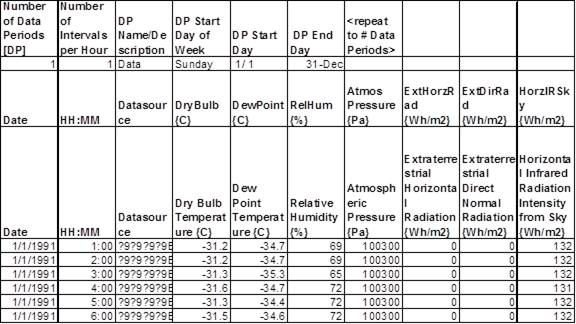
\includegraphics[width=0.9\textwidth, height=0.9\textheight, keepaspectratio=true]{media/image016.png}
\caption{Illustration of Building North Axis \protect \label{fig:illustration-of-building-north-axis}}
\end{figure}

\emph{Zone information:}

\begin{enumerate}
\def\labelenumi{\arabic{enumi}.}
\tightlist
\item
  \emph{Wall height}: In a simple model, one should make all the walls the same height. Then, the simple, 1 zone model can entirely enclose the space. In more complex models, you may resize each wall accordingly.
\end{enumerate}

\emph{Surface information:}

1.~~ \emph{Base} \emph{Surface Type:} Heat Transfer/Heat Storage Surfaces may be of the following types: wall, floor, roof, internal mass, or subsurface

2.~~ \emph{Construction:} The type of construction of the surface (see previous table).

\emph{Subsurface information:}

1.~~~~\emph{Subsurfaces} are Windows, Doors or GlassDoors

2.~~ \emph{Area:} Area of the subsurface.

3.~~ \emph{Reveal:} For windows only, the distance it is inset from the outside surface of a wall. For simplicity, put all the windows in the same physical plane as the wall they are on.

For the single zone model, the following figure is a schematic representation of a one zone representation. The figure shows the length of all ``base'' surfaces and the areas of all ``subsurfaces'' (windows). Doors are shown and may be entered, if desired. In the table (Table~\ref{table:compilation-of-surface-information-for}), the surfaces are numbered counter-clockwise around the zone beginning at the lower left corner of the figure. ~This table is the minimum required zone information compiled by the user. A few simple conventions should be followed to facilitate the construction of zone information tables:

1.~~ Number all surfaces in order counter-clockwise around the zone.

2.~~ Keep the subsurfaces with the base surface on which they are located.

3.~~ Specify \emph{lengths} for base surfaces and areas for subsurfaces and internal mass.

4.~~~~Specify the roof and floor as rectangles of the correct size.

\begin{figure}[hbtp] % fig 17
\centering
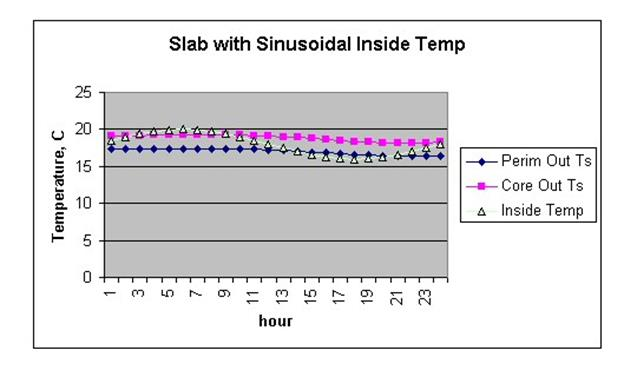
\includegraphics[width=0.9\textwidth, height=0.9\textheight, keepaspectratio=true]{media/image017.jpg}
\caption{Schematic of One Zone Model with Exterior Wall length and Window Areas. \protect \label{fig:schematic-of-one-zone-model-with-exterior}}
\end{figure}

\textbf{Full Building -- 1 Zone model}

% table 5
\begin{longtable}[c]{p{1.2in}p{1.2in}p{1.2in}p{1.2in}p{1.2in}}
\caption{Compilation of Surface Information for the One Zone Model \label{table:compilation-of-surface-information-for}} \tabularnewline
\toprule 
Surface & type & construction & Length \{m\} & Area \{m  \} \tabularnewline
\midrule
\endfirsthead

\caption[]{Compilation of Surface Information for the One Zone Model} \tabularnewline
\toprule 
Surface & type & construction & Length \{m\} & Area \{m  \} \tabularnewline
\midrule
\endhead

1 & exterior wall & Medium Exterior Wall & 15.25 & ~ \tabularnewline
2 & window & Double Pane Window & ~ & 5.62 \tabularnewline
3 & exterior wall & Medium Exterior Wall & 4.9 & ~ \tabularnewline
4 & window & Double Pane Window & ~ & 3.9 \tabularnewline
5 & exterior wall & Medium Exterior Wall & 34.44 & ~ \tabularnewline
6 & window & Double Pane Window & ~ & 33.7 \tabularnewline
7 & exterior wall & Medium Exterior Wall & 13.2 & ~ \tabularnewline
8 & window & Double Pane Window & ~ & 9.44 \tabularnewline
9 & exterior wall & Medium Exterior Wall & 10.4 & ~ \tabularnewline
10 & window & Double Pane Window & ~ & 7.58 \tabularnewline
11 & exterior wall & Medium Exterior Wall & 20 & ~ \tabularnewline
12 & window & Double Pane Window & ~ & 10.5 \tabularnewline
13 & exterior wall & Medium Exterior Wall & 12 & ~ \tabularnewline
14 & window & Double Pane Window & ~ & 7.58 \tabularnewline
15 & exterior wall & Medium Exterior Wall & 20 & ~ \tabularnewline
16 & window & Double Pane Window & ~ & 17.66 \tabularnewline
17 & exterior wall & Medium Exterior Wall & 6.1 & ~ \tabularnewline
18 & window & Double Pane Window & ~ & 4.7 \tabularnewline
19 & exterior wall & Medium Exterior Wall & 3.1 & ~ \tabularnewline
20 & exterior wall & Medium Exterior Wall & 6.1 & ~ \tabularnewline
21 & window & Double Pane Window & ~ & 3.71 \tabularnewline
22 & exterior wall & Medium Exterior Wall & 23 & ~ \tabularnewline
23 & window & Double Pane Window & ~ & 19.39 \tabularnewline
24 & exterior wall & Medium Exterior Wall & 15.24 & ~ \tabularnewline
25 & window & Double Pane Window & ~ & 7.8 \tabularnewline
26 & exterior wall & Medium Exterior Wall & 38 & ~ \tabularnewline
27 & window & Double Pane Window & ~ & 31 \tabularnewline
28 & roof & Medium Roof/Ceiling & Equivalent area (square) & 1250.1 \tabularnewline
29 & floor & Medium Floor & Equivalent area (square) & 1250.1 \tabularnewline
30 & internal mass & Medium Partitions & ~ & 956.9 \tabularnewline
31 & internal mass & Medium/Heavy Partitions & ~ & 1757.7 \tabularnewline
\bottomrule
\end{longtable}

The column headings in the previous table have the following meanings:

\textbf{Type:}~ A shortened notation for the surface type in EnergyPlus to differentiate between heat storage surfaces and various types of heat transfer surfaces.

\textbf{Construction:}~ A name for the surface construction types.

\textbf{Length:}~ The length of base surfaces (i.e.~Exterior Walls).

\textbf{Area:}~ The area of subsurfaces (windows), roofs, floors.

\subsection{\emph{Step 4}: Compile Internal Space Gain Data}\label{step-4-compile-internal-space-gain-data}

People, lights, equipment, outside air infiltration and ventilation all constitute ``internal gains'' for the thermal zone. These gains are described to EnergyPlus as a \emph{design or} \emph{peak} level with a \emph{schedule} that specifies a fraction of the peak for each hour. The peak level is calculated by the user. Table~\ref{table:internal-gain-data}. Internal Gain Data shows the internal loads for a single zone model of Ft. Monmouth and the schedule named to specify the hourly load.

% table 6
\begin{longtable}[c]{@{}llll@{}}
\caption{Internal Gain Data \label{table:internal-gain-data}} \tabularnewline
\toprule 
Zone & Gain Type & Size & Schedule \tabularnewline
\midrule
\endfirsthead

\caption[]{Internal Gain Data} \tabularnewline
\toprule 
Zone & Gain Type & Size & Schedule \tabularnewline
\midrule
\endhead

1 & People & 205 & Office occupancy \tabularnewline
~ & Lights & 26360 W & Office lighting \tabularnewline
~ & ZoneInfiltration & .75 m  /sec & Constant \tabularnewline
\bottomrule
\end{longtable}

The column headings in the table have the following meanings:

\textbf{Gain Type:}~ The code used to differentiate between various types of internal gains.

\textbf{Size:}~ The peak load. This is the actual size of the load for every hour that the schedule specifies ``100\%''.

\textbf{Schedule:}~ The hourly schedule that specifies the percentage of peak load for each hour of the day.

\textbf{HVAC:} Using the Compact HVAC models, purchased air can be used to calculate the energy needs of the building.

As the following figure shows, the equivalent area floor/roof does not fit in the building perimeter. As an exercise, you might reconfigure both floor and roof to be a polygonal shape and compare results.

\begin{figure}[hbtp] % fig 18
\centering
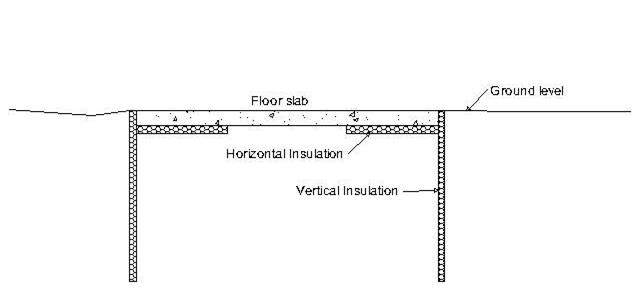
\includegraphics[width=0.9\textwidth, height=0.9\textheight, keepaspectratio=true]{media/image018.png}
\caption{Full Building - Adult Education Center \protect \label{fig:full-building-adult-education-center}}
\end{figure}

As an adjunct to the previous schematic layout for the one zone approach, the following figure shows the same building but with IP units:

\begin{figure}[hbtp] % fig 19
\centering
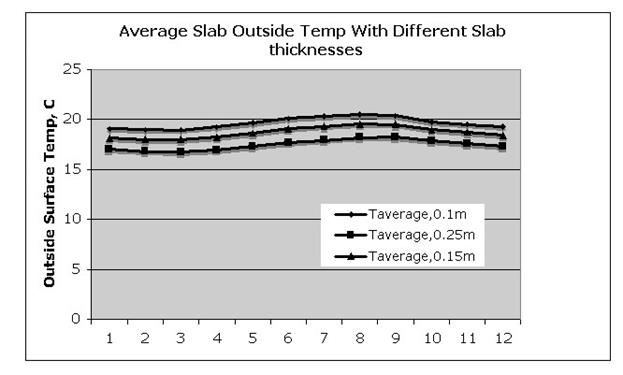
\includegraphics[width=0.9\textwidth, height=0.9\textheight, keepaspectratio=true]{media/image019.jpg}
\caption{Schematic for One Zone Building - IP Units \protect \label{fig:schematic-for-one-zone-building-ip-units}}
\end{figure}
